
\subsection{Data Model}

In the context of our work, the data we are considering can be seen as both \emph{static} and \emph{volatile} data, as we are considering a bank system application that, on the one hand, it contains all the \emph{static} information related to it about the cards, clients, accounts, among others, that a bank typically gathers. And, on the other hand, it is a system where transactions made by clients with their cards at ATMs, POS terminals, etc., are continuously occurring and received in a streaming manner: the \emph{volatile} data.\\

Therefore, due to this nature of the data, we consider a \emph{continuously evolving database} paradigm, where data can be both stable and volatile. Even though 
evolving databases can be implemented according to any approach, we decided to use the property graph data model (see \ref{prelim:graphdatamodel-pg}). Our property graph is a \emph{continuously evolving data graph}, which has a persistent (\emph{stable}) as well as non persistent (\emph{volatile}) relations. Stable relations correspond to edges occurring in standard graph databases while volatile relations are edges arriving in data streams during a set time interval.\\

The property graph data model provides us many benefits: (i) it is a simple and easy method to represent entities and their relationships in the form of graphs; (ii) it is a convenient model to represent dynamic data sources, in our case the continuously occurring relations between cards and ATMs; (iii) and it provides us a direct way to model queries related with fraud pattern matching. Finally, mention that we used \texttt{Neo4j} (see \ref{prelim:graphdbsystem-neo4j}) as the graph database management system to implement our property graph data model. \\

\subsubsection*{Design of the Property Graph Data Model}

In what follows we describe the design of our property graph taken data model. Due to the confidential and private nature of bank data, it was impossible to find a real bank dataset nor a real bank data model. In this regard, we developed our own proposal of a bank database model taking as standard reference the \emph{Wisabi Bank Dataset}, which is a fictional banking dataset publicly available in the Kaggle platform\cite{wisabi-bank-dataset}.\\

\begin{figure}[h]
  \centering
  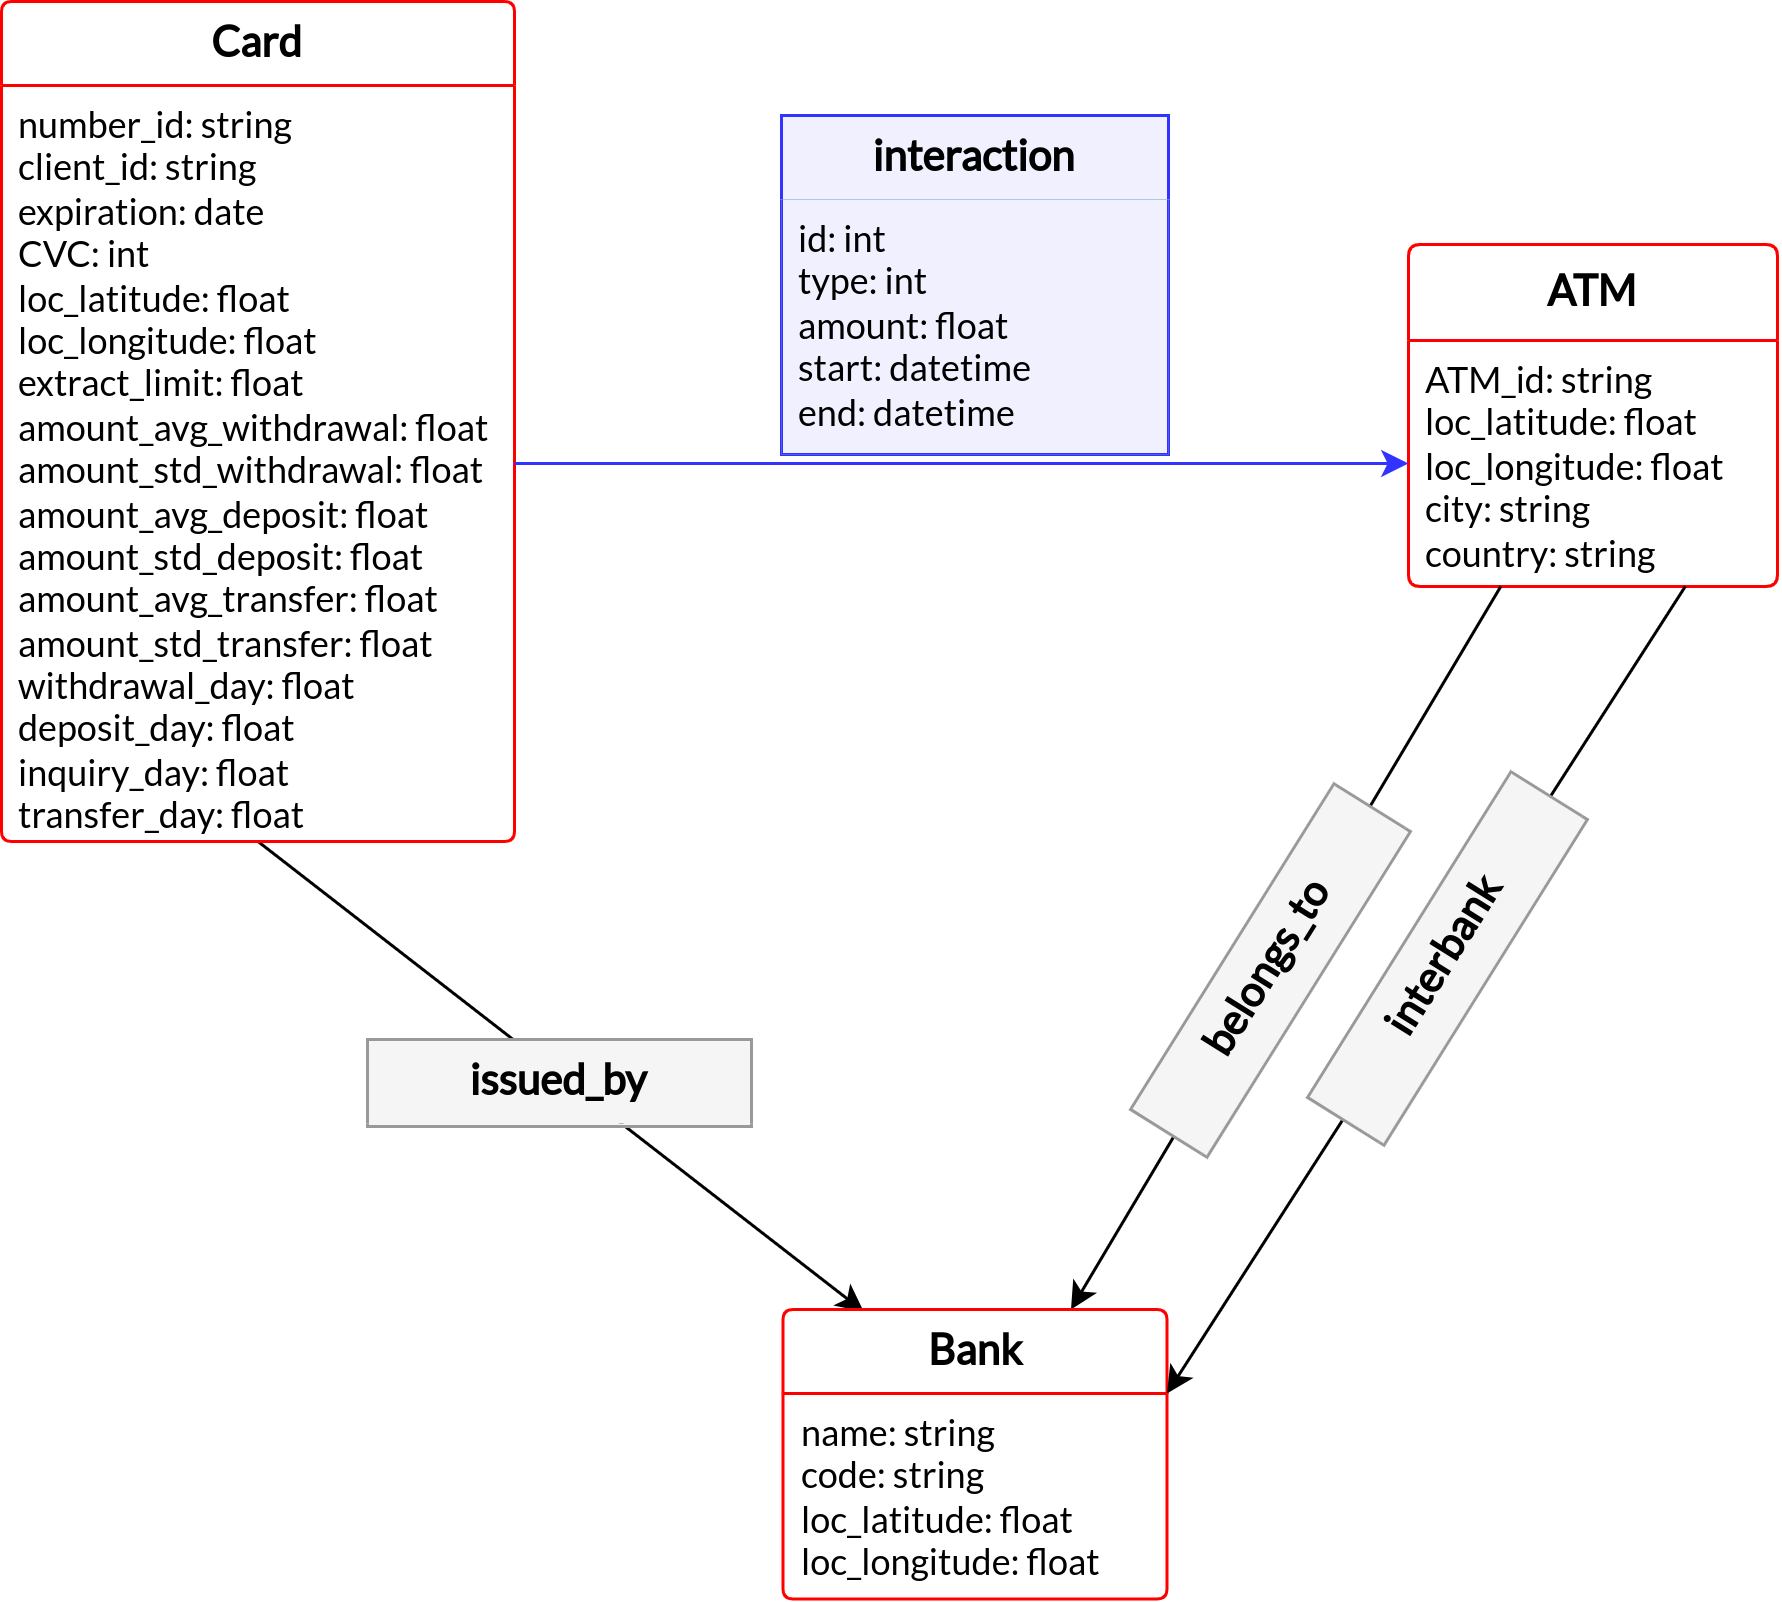
\includegraphics[scale = 0.8]{images/1-DataModel/PG-behavior-complete.png}
  \caption{Complete property graph bank data model representation}
  \label{img:pg-complete}
\end{figure}

The proposed property graph data model is represented in Figure \ref{img:pg-complete}, consisting on both the stable and volatile property subgraphs merged.
The main difference and the primary reason for this separation is the semantics with which we intentionally define each of the subgraphs: the stable will be understood like a fixed static bank database, whereas the volatile will be understood as the data model to define the transactions, as continuous interactions between the entities of the model, which will not be permanently saved, but instead, only for a certain window of time under the mission of detecting anomalous bank operations. 
Note that we will only model the transaction interaction in the volatile subgraph, with no incidence in any other element of the architecture.
This separation will allow us to have a really simple and light property graph schema single-centered on the transactions with the minimal needed information 
(mostly identifiers of the entities and transaction links) and another, the stable, acting as a traditional bank database schema, from which to obtain the information details of the entities.
%%%

\paragraph*{Stable Property Graph\\\\}\label{section:stable-pg}

Taking into account the reference dataset model, we designed a simplified version, as shown in Figure \ref{img:pg-stable-def}, with the focus on representing and modeling card-ATM interactions. On it, the defined entities, relations and properties modeling the bank database are reduced to the essential ones, which are enough to create a relevant and representative bank data model, sufficient for the purposes of our work. Another option for the property graph data model representing a more common bank data model could be the one we defined in Figure \ref{img:pg-stable-big}, which intents to capture the data that a bank system database typically gathers. It consists of a more complete and possibly closer to reality data model, although unnecessarily complex for our objectives.\\

\begin{figure}[H]
  \centering
  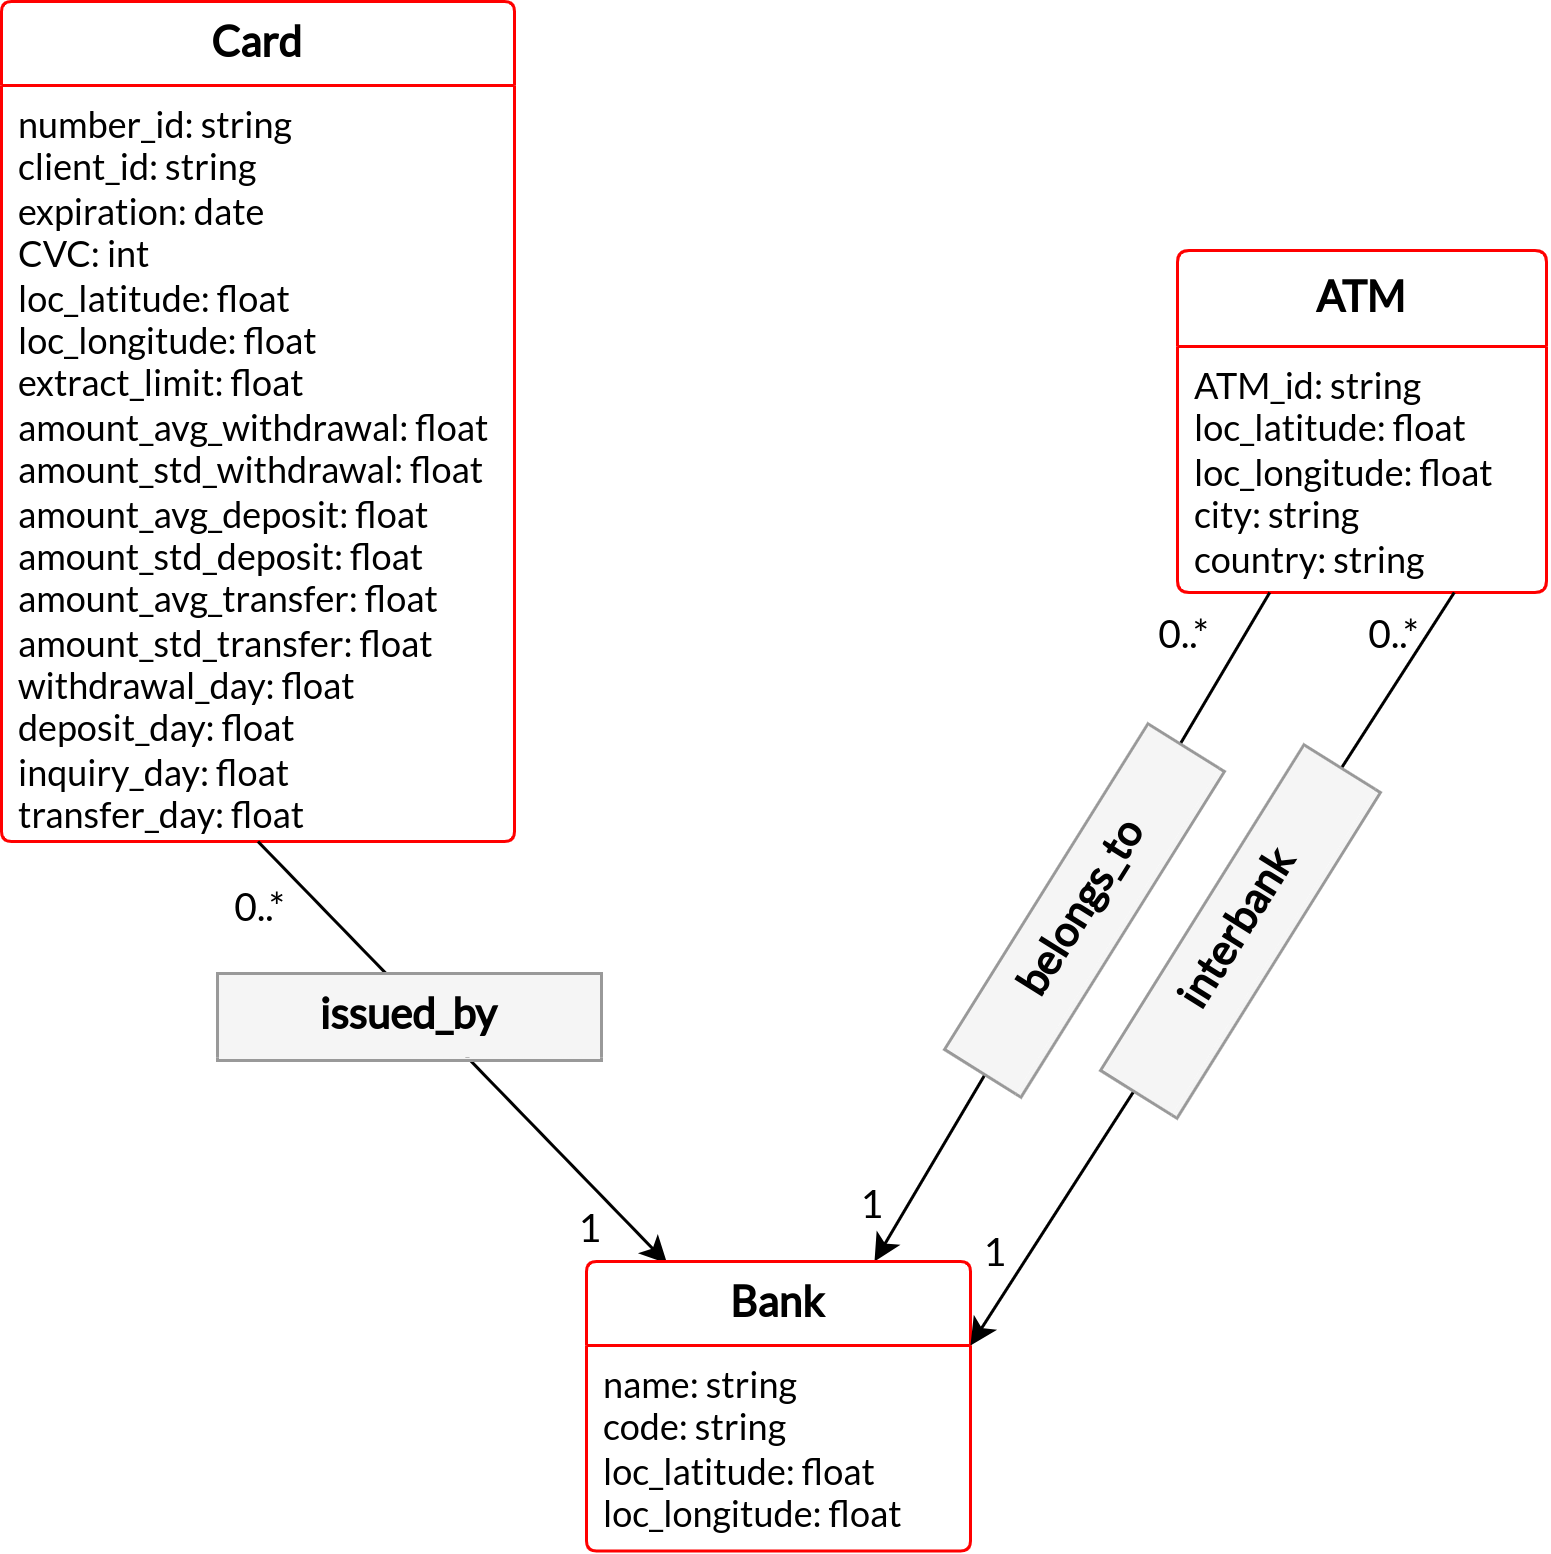
\includegraphics[scale = 0.8]{images/1-DataModel/PG-stable-behavior-cards.png}
  \caption{\emph{Stable} property graph bank data model}
  \label{img:pg-stable-def}
\end{figure}

As a result, our definitive stable property graph model contains three node entities: \texttt{Bank}, \texttt{Card} and \texttt{ATM}, and three relations: \texttt{issued\_by} associating \texttt{Card} entities with the \texttt{Bank} entity, and \texttt{belongs\_to} and \texttt{interbank} associating the \texttt{ATM} entities with the \texttt{Bank} entity.\\

% Bank
\paragraph{\texttt{Bank}\\\\}

The \texttt{Bank} entity represents the bank we are considering in our system. Its properties consist
on the bank \emph{name}, its identifier \emph{code} and the location
of the bank headquarters, expressed in terms of \emph{latitude} and \emph{longitude}
coordinates, as seen in Table \ref{table:bank-node-properties}.\\
  
\begin{table}[H]
    \centering
      \begin{tabular}{|l|l|}
      \hline
      \textbf{Name}        & \textbf{Description and value}                                      \\ \hline
      \texttt{name}         & Bank name                                                 \\ \hline
      \texttt{code}         & Bank identifier code                                      \\ \hline
      \texttt{loc\_latitude}  & Bank headquarters GPS-location latitude                   \\ \hline
      \texttt{loc\_longitude} & Bank headquarters GPS-location longitude                  \\ \hline
      \end{tabular}
    \caption{Bank node properties}
    \label{table:bank-node-properties}
\end{table}

\paragraph{\texttt{ATM}\\\\}

The \texttt{ATM} entity represents the Automated Teller Machines (ATM) that either belong to the bank's network or that the bank can interact with.
% Potential possible generalization of the ATM entity to a POS entity
For the moment, this entity is understood as the classic ATM, however note that this entity could be potentially generalized to a \emph{Point-Of-Sale} (POS) entity, allowing a more general kind of interactions apart from the current Card-ATM interaction, where also POS terminal transactions could be included apart from the ATM ones. We distinguish two different kinds of ATMs, depending on their relation with the bank:
\begin{itemize}
  \item \textbf{Internal \texttt{ATMs}}: ATMs owned and operated by the bank. They are fully integrated within the
  bank's network. Modeled with the \texttt{belongs\_to} relation.
  \item \textbf{External \texttt{ATMs}}: These ATMs, while not owned by the bank, are still accessible for the bank
  customers to perform transactions. Modeled with the \texttt{interbank} relation. 
\end{itemize}

Both types of ATMs are considered to be of the same type of \texttt{ATM} node. Their difference is modeled as their relation with the bank instance: \texttt{belongs\_to} for the internal ATMs and \texttt{interbank} for the external ATMs.\\

\begin{table}[H]
    \centering
    \begin{tabular}{|l|l|}
    \hline
    \textbf{Property}        & \textbf{Description}                                      \\ \hline
    \texttt{ATM\_id}      & ATM unique identifier                             \\ \hline
    \texttt{loc\_latitude}  & ATM GPS-location latitude           \\ \hline
    \texttt{loc\_longitude} & ATM GPS-location longitude          \\ \hline
    \texttt{city}         & ATM city location                         \\ \hline
    \texttt{country}      & ATM country location                       \\ \hline
    \end{tabular}
    \caption{ATM node properties}
    \label{table:atm-node-properties}
\end{table}

The \texttt{ATM} node properties consist on the ATM unique identifier \emph{ATM\_id}, its location, expressed in terms of \emph{latitude} and \emph{longitude} coordinates, and the \emph{city} and 
\emph{country} in which it is located, as seen in Table \ref{table:atm-node-properties}.
Note that the last two properties are somehow redundant, considering that location coordinates
are already included. In any case both properties are maintained since their inclusion provides a more explicit and direct description of the location of the ATMs, which will be of special interest for some of the card anomalous patterns that will be considered.\\

\paragraph{\texttt{Card}\\\\}

The \texttt{Card} node represents the cards of the clients in the bank system. The \texttt{Card} node type properties, as depicted in Table
\ref{table:card-node-properties}, consist on the card unique 
identifier \emph{number\_id}, the associated client unique identifier \emph{client\_id}, the card validity expiration date \emph{expiration}, the Card Verification Code, \emph{CVC}, the coordinates of the associated client habitual residence address \emph{loc\_latitude} and 
\emph{loc\_longitude} and the \emph{extract\_limit} property, which represents the limit on the amount of money it can be extracted with the card on a single withdrawal, related with the the amount of money a person owns. These last two properties are of special interest for some future card fraud patterns to be considered. In the first case related with interactions far from the client's habitual residence address and in the second with unusually frequent or very high expenses interactions.\\

Finally, it contains the properties related with the \emph{behavior} of the client, representing the usual comportment of a client in regard with its ATM usage: \emph{amount\_avg\_withdrawal}, \emph{amount\_std\_withdrawal}, \emph{amount\_avg\_deposit}, 
\emph{amount\_std\_deposit}, \emph{amount\_avg\_transfer},\\  \emph{amount\_std\_transfer}, \emph{withdrawal\_day}, \emph{deposit\_day}, \emph{transfer\_day} and \emph{inquiry\_day}.
They are metrics representing the behavior of the owner of the Card, and they are included as properties as we think they could be of interest to allow the detection of some kinds of anomalies related with anomalous client's behavior in the future.

\begin{table}[H]
    \centering
    \begin{tabular}{|l|l|}
    \hline
    \textbf{Name}        & \textbf{Description and value}                                          \\ \hline
    \texttt{number\_id}   & Card unique identifier                               \\ \hline
    \texttt{client\_id}   & Client unique identifier                               \\ \hline
    \texttt{expiration}   & Card validity expiration date                      \\ \hline
    \texttt{CVC}          & Card Verification Code                                      \\ \hline
    \texttt{extract\_limit} & Card money amount extraction limit    \\ \hline
    \texttt{loc\_latitude}  & Client's habitual address GPS-location latitude                         \\ \hline
    \texttt{loc\_longitude} & Client's habitual address GPS-location longitude                        \\ \hline
    \end{tabular}
    \caption{Card node properties}
    \label{table:card-node-properties}
\end{table}

In the proposed property graph bank data model the client is completely anonymized in the system (no name, surname, age, or any other confidential details) by using only a \emph{client\_id}. Currently, \emph{client\_id} is included in the \texttt{Card} node type for completeness. However, it could be omitted for simplicity, as we assume a one-to-one relationship between a card and a client for the purposes of our work -- each card is uniquely associated with a single client, and each client holds only one card. Thus, the \emph{client\_id} is not essential at this stage but is retained in case the database model is expanded to support clients with multiple cards or cards shared among different clients.

\begin{figure}[H]
  \centering
  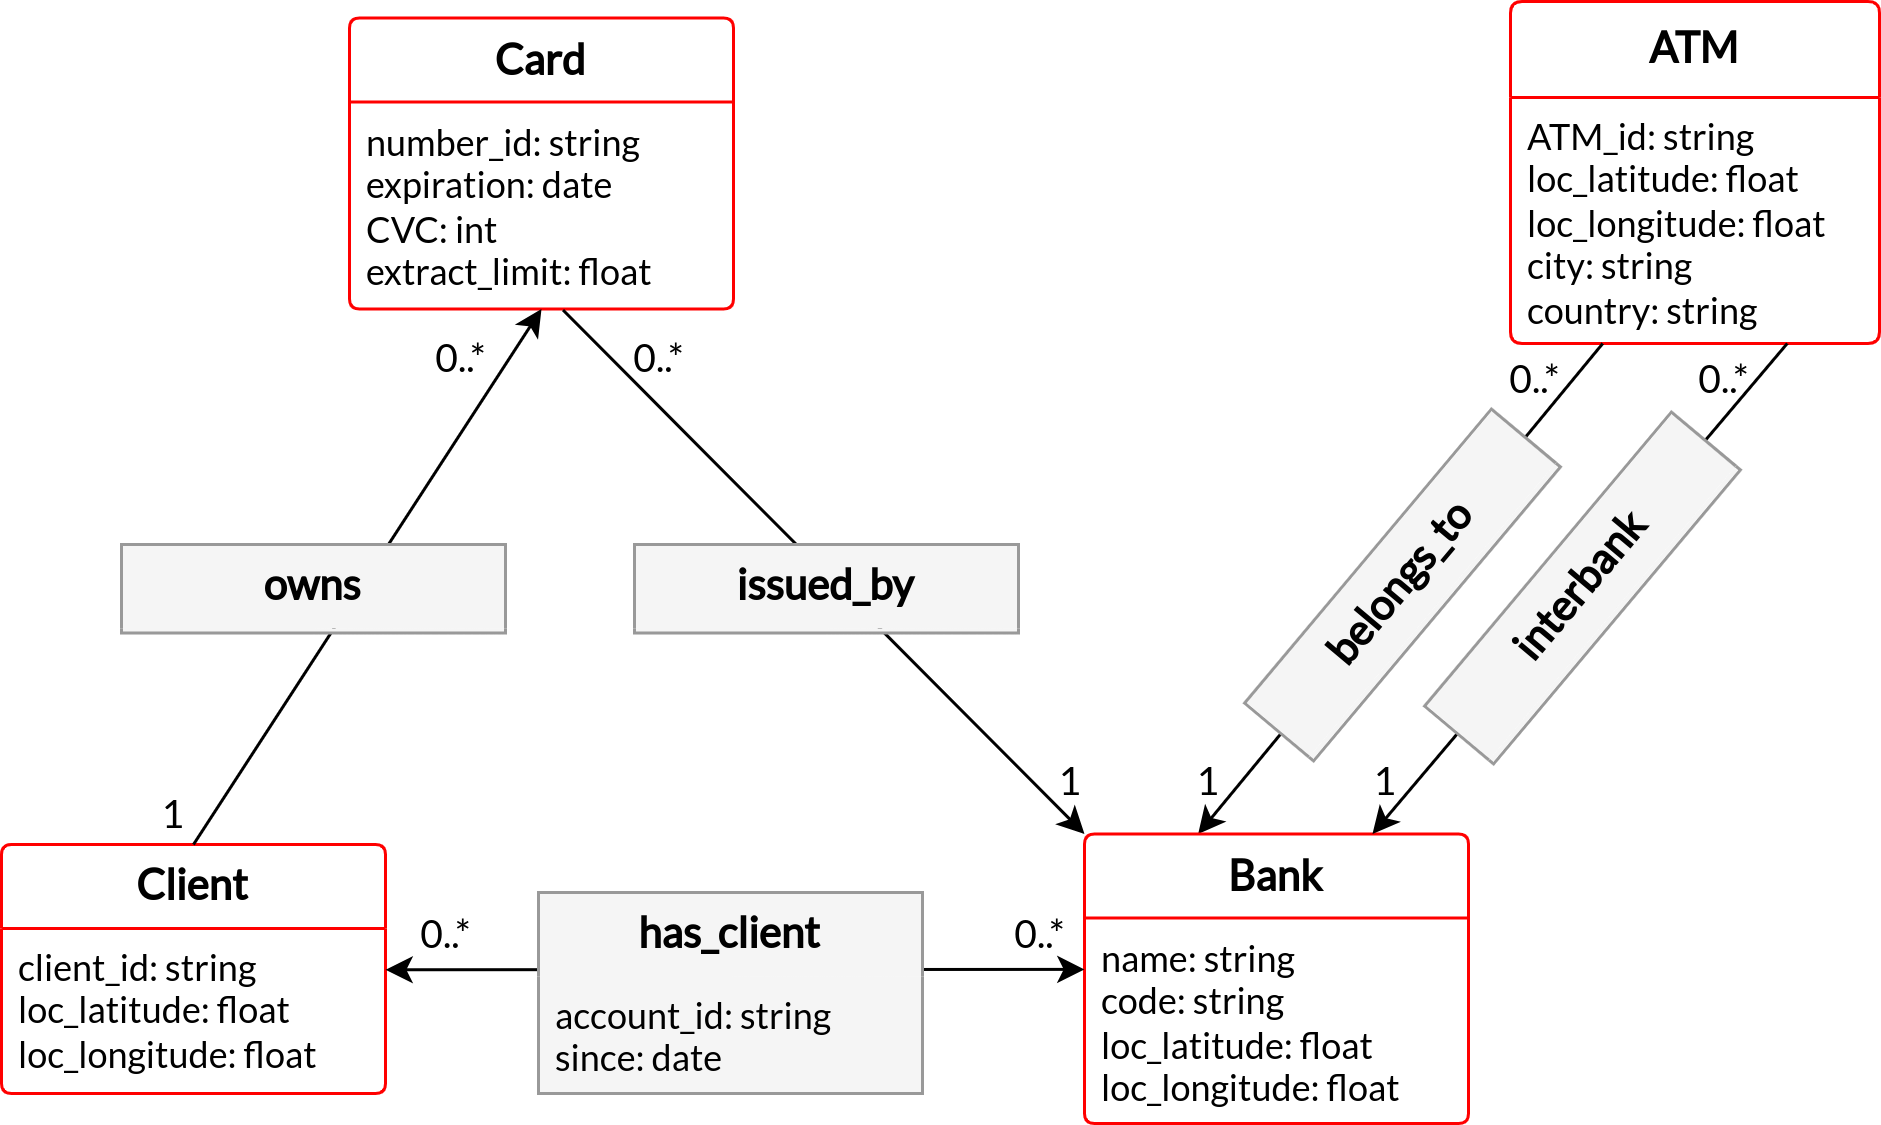
\includegraphics[scale = 0.7]{images/1-DataModel/PG-stable-edit-cardinal.png}
  \caption{Alternative - A more complex stable property graph bank data model. It consists of four node entities: \texttt{Bank}, \texttt{ATM}, \texttt{Client} and \texttt{Card} with their respective properties, and the corresponding relationships between them. The relations are: a directed relationship from \texttt{Client} to \texttt{Card} \texttt{owns} representing that a client can own multiple credit cards and that a card is owned by a unique client, then a bidirectional relation \texttt{has\_client} between \texttt{Client} and \texttt{Bank}; representing bank accounts of the clients in the bank. The relation between \texttt{Card} and \texttt{Bank} to represent that a card is \texttt{issued\_by} the bank, and that the bank can have multiple cards issued. Finally, the relations \texttt{belongs\_to} and \texttt{interbank} between the \texttt{ATM} and \texttt{Bank} entities, representing the two different kinds of ATMs depending on their relation with the bank; those ATMs owned and operated by the bank and those that, while not owned by the bank, are still accessible for the bank customers to perform transactions. This model allows a more elaborated representation of what a bank system database is. As it can be seen it represents clients as an independent entity from the \texttt{Card} entity, and it also allows to represent bank accounts through the relation between the \texttt{Client} and \texttt{Bank} entities. }
  \label{img:pg-stable-big}
\end{figure}


\paragraph*{Volatile Property Graph\\\\}\label{section:volatile-pg}

The volatile property graph consists on an abstraction of the property graph model to describe the interactions between the cards and the ATMs in the bank system. These interactions are going to be continuously occurring and arriving to our system as data stream.\\

The proposed property graph, represented on Figure \ref{img:pg-volatile}, is a subgraph of the original bank property graph model (Figure \ref{img:pg-complete}). It contains the \texttt{Card} and \texttt{ATM} entities with the minimal information needed to identify them -- \emph{number\_id} and \emph{ATM\_id}, Card and ATM identifiers, respectively -- between which the interaction occurs, along with additional details related to the interaction. Those identifiers are enough to be able to recover, if needed, the whole information about the specific \texttt{Card} or \texttt{ATM} entity in the stable property graph. In addition, it contains the \texttt{interaction} relationship between the \texttt{Card} and the \texttt{ATM} nodes. The \texttt{interaction} relation contains as properties (see table \ref{table:interaction-relation-properties}): \emph{id} as the interaction unique identifier, \emph{type} which describes the type of the interaction (withdrawal, deposit, balance inquiry or transfer), \emph{amount} describing the amount of money involved in the interaction in the local currency considered, and finally, \emph{start} and \emph{end} which define the interaction \emph{datetime} start and end moments, respectively. 

\begin{figure}[h]
    \centering
    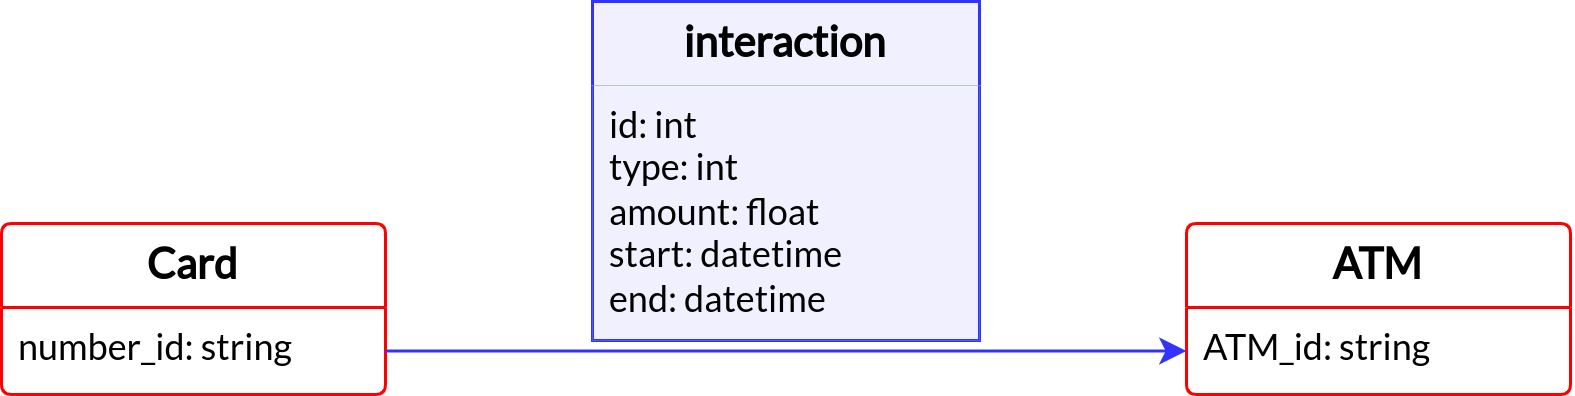
\includegraphics[scale = 0.8]{images/1-DataModel/schema-volatile.png}
    \caption{Volatile Property Graph Data Model}
    \label{img:pg-volatile}
\end{figure}

\begin{table}[H]
    \centering
    \begin{tabular}{|l|l|}
    \hline
    \textbf{Property}        & \textbf{Description}                                      \\ \hline
    \texttt{id}      & Interaction/Transaction unique identifier                             \\ \hline
    \texttt{type}  & Transaction type: withdrawal, deposit, balance inquiry or transfer           \\ \hline
    \texttt{amount} & Money amount involved in the transaction          \\ \hline
    \texttt{start}         & Transaction start time moment                         \\ \hline
    \texttt{end}      & Transaction end time moment                     \\ \hline
    \end{tabular}
    \caption{Interaction relation properties}
    \label{table:interaction-relation-properties}
\end{table}

A key aspect that we consider in our data model is the division of the \texttt{interaction} relation in two edges -- the \emph{opening} and the \emph{closing} edges -- both forming a single \texttt{interaction} relation. The \emph{opening} edge (Figure \ref{img:opening-edge-1}) will be the indicator of the beginning of a new interaction between a Card and a ATM. It contains the values of the properties related with the starting time \emph{start}, the interaction \emph{type} as well as the \emph{id}. The \emph{closing} edge (Figure \ref{img:closing-edge-1}) will indicate the end of the interaction, completing the values of the rest of the properties of the interaction: \emph{end} and \emph{amount}.

\begin{figure}[H]
  \centering
  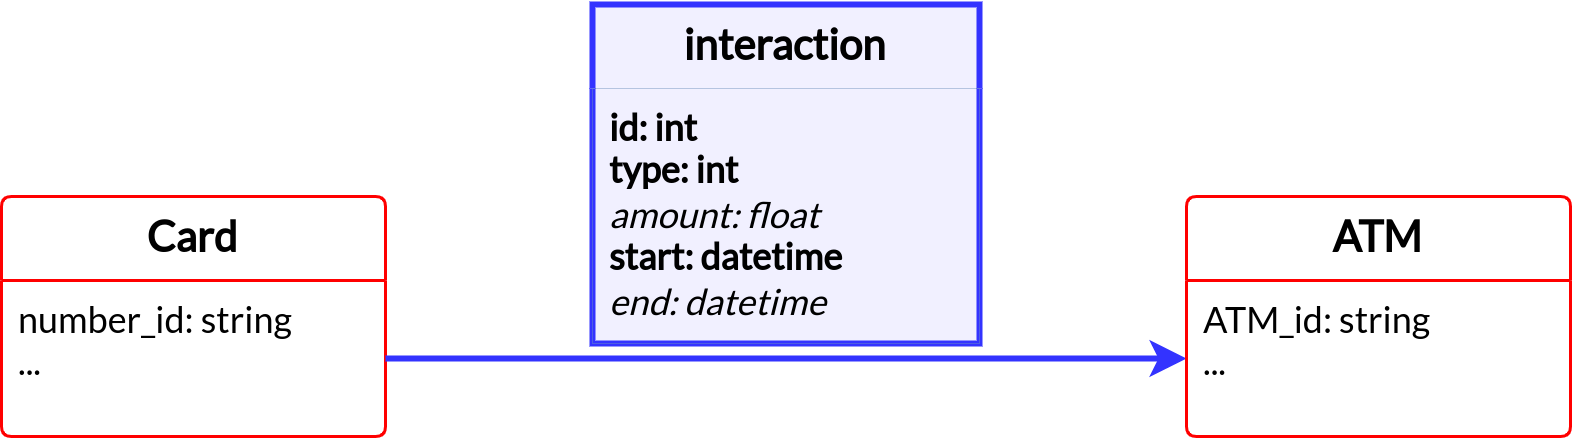
\includegraphics[scale = 0.8]{images/1-DataModel/2-edges-tx-tfm.png}
  \caption{\emph{Opening} interaction edge}
  \label{img:opening-edge-1}
\end{figure}

With this division of the \texttt{interaction} relation in two edges we are simulating that for each transaction, our system receives an initial message when the transaction starts and a final message once the transaction is finished on the ATM. This can be a key aspect in our system, since it can allow us to develop a system that is able not only to detect anomalous scenarios on interactions that have already been produced/closed, but also to act in real time before the anomalous transaction detected has actually occurred.

\begin{figure}[H]
  \centering
  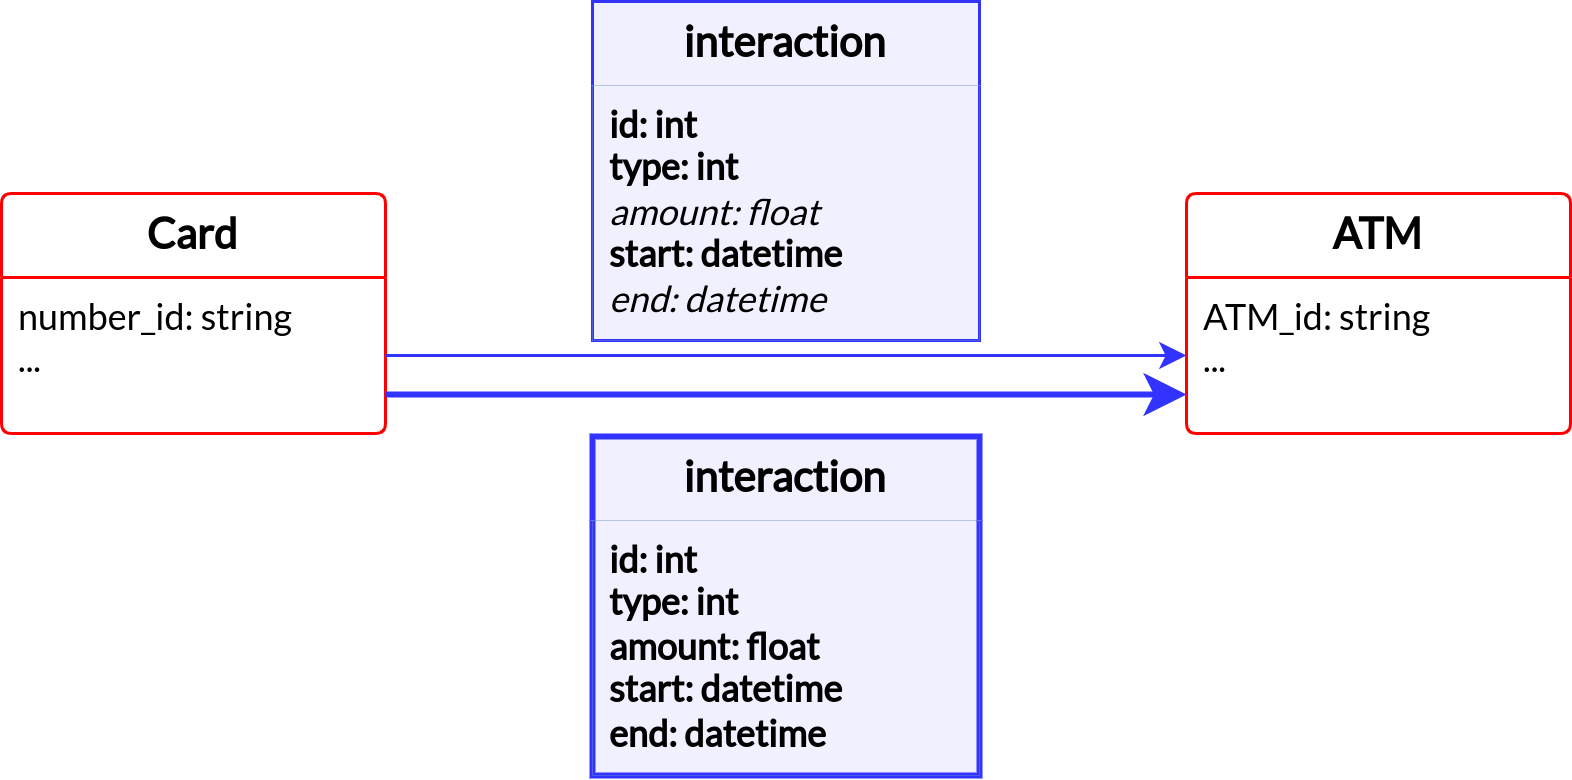
\includegraphics[scale = 0.8]{images/1-DataModel/2-edges-tx-tfm-1.png}
  \caption{\emph{Closing} interaction edge}
  \label{img:closing-edge-1}
\end{figure}
